\documentclass{l3proj}
\usepackage{lscape}

\makeatletter
\newcommand\ackname{Acknowledgements}
\if@titlepage
  \newenvironment{acknowledgements}{%
      \titlepage
      \null\vfil
      \@beginparpenalty\@lowpenalty
      \begin{center}%
        \bfseries \ackname
        \@endparpenalty\@M
      \end{center}}%
     {\par\vfil\null\endtitlepage}
\else
  \newenvironment{acknowledgements}{%
      \if@twocolumn
        \section*{\abstractname}%
      \else
        \small
        \begin{center}%
          {\bfseries \ackname\vspace{-.5em}\vspace{\z@}}%
        \end{center}%
        \quotation
      \fi}
      {\if@twocolumn\else\endquotation\fi}
\fi
\makeatother

\begin{document}
\title{GIM - Team G Instant Messenger}
\author{Ewan Baird \\
Heather Hoaglund-Biron \\
Gordon Martin \\
James McMinn}
\date{21 March 2011}
\maketitle

\begin{abstract}
GIM is a client-server instant messaging application implemented in the Java programming language. Comparable to many other similar programs, GIM allows users to communicate over a network with text-based messages, using a protocol we developed from scratch. This dissertation discusses the process of developing GIM from the initial problem definition through to completion.
\end{abstract}

\begin{acknowledgements}
Thanks to Colin Perkins for supervising this project, and being the voice of reason in those rare moments when panic set in.

For his excellent art work, we would like to thank our fellow student Matt Roszak. Without any brief, he provided an excellent logo and icon set for us, giving up his spare time in the process.

We would also like to thanks all of those who helped test the program, even in those early stages without the pretty GUI.
\end{acknowledgements}

\educationalconsent

\setcounter{tocdepth}{1}
\tableofcontents

\chapter{Introduction}
\label{introduction}

\section{Introduction}

Instant messengers are an easy, fast way to communicate over the Internet. Basic instant messengers allow users to type messages to each other on separate computers and have those messages immediately show on the screen, like instant email. More advanced systems have features like audio and video communication. These days instant messengers are becoming more popular, given the way the Internet is helping people from all over the world connect with one another. This has led to an increased demand for quick and easy communication.

These days, it's difficult to be original when developing an instant messenger. Programs like Skype\footnote{\texttt{http://www.skype.com/}}, AIM\footnote{\texttt{http://www.aim.com/}} and Windows Live Messenger\footnote{\texttt{http://explore.live.com/}} are popular, especially with the younger generation. There are many kinds of instant messengers out there, the most prominent of which are always competing against each other to have the newest and most intriguing features.

This project is not about joining that competition. Instead, we are using this opportunity to explore what it's like to create an instant messenger from the ground up. As we are part of the younger generation, we use instant messengers almost daily, and it's interesting to be able to go behind the scenes and discover how they work for ourselves.

The instant messenger model that we decided to use consists of a server, any number of clients, and a set of rules defining how the server and clients talk to each other, called a protocol. A user of the program is essentially interacting with a client, and the clients interact with each other through the server. That communication is structured using the protocol.

Instead of using the protocol and server of an existing instant messenger and focusing on the client, we decided to create the entire system ourselves. This way we're able to learn more about the whole process of creating such a program. We have divided ourselves into two smaller groups: two of us to do the networking and make the server, and the other two to make the client, including the user interface, or UI.

This report is meant for the Computing Science professors at Glasgow University, fellow Computing Science students, and anyone with an interest in instant messaging or the process of completing a large-scale Computing Science project.

The structure of this report is as follows. In Chapter 1, we have this introduction, the problem definition, and an overview of the requirements. Chapter 2 covers the design of the protocol, client, server, and overall networking. In Chapter 3 is a discussion of our implementation of the client and server. Chapter 4 covers evaluation of our finished product, and Chapter 5 is a conclusion and reflective of what we learned.


\section{Problem Definition}
The following was our given problem definition\footnote{\texttt{http://fims.moodle.gla.ac.uk/file.php/129/1243.pdf}}:

\begin{quote}
Instant messaging systems such as Jabber\footnote{\texttt{http://www.jabber.org/}}, AIM, ICQ\footnote{\texttt{http://www.icq.com/}} and IRC\footnote{\texttt{http://www.irc.org/}} have become popular in the last few years. The aim of the project is to build a simple instant messaging system, written in Java\footnote{\texttt{http://www.oracle.com/technetwork/java/index.html}}, to develop your understanding of networked systems and programming.

The group will be required to develop both an instant messaging client and server, and to design the network protocol they use to communicate. The server should accept connections from an arbitrary number of clients. Clients will have a graphical user interface, and should be able to accept and receive text-based messages, to indicate if the user is busy, available or idle, and to convey usernames and other details.

The project involves network and user-interface programming. It would suit a group with an interest in low-level systems design and implementation issues.
\end{quote}

Despite the fact the above problem definition says we have to develop the client, server, and protocol, we were told we could also construct the system using the protocol of another existing instant messenger, like IRC or Windows Live Messenger. In that case, we would focus more on the development of the client. Instead, we opted to create the whole thing ourselves, since it would give us more control and we would be able to learn more about the entire process of creating an instant messenger.

The problem definition also states that we should at least have text-based messages, statuses (online, offline, etc), and usernames. We decided to expand on this, to make the final product as complete a messenger as possible. We added smileys (or emoticons), small pictures that depict emotions in messages, personal messages, display pictures for each user, and more.

It wasn't explicitly stated, but we had to decide how to structure the users: whether users should have ``contacts,'' whether messaging should be chatroom-style, and whether there should be one-on-one conversations, group conversations, or both. We chose to do a combination, in that users may have contacts and one-on-one conversations, but may also join, create, and invite other users to group chatrooms. We decided this combined our favorite aspects of two major instant messengers: the personal conversations of programs like Windows Live Messenger and the community-oriented chatrooms of IRC.



\chapter{Requirements}
\label{requirements}

\section{Problem Definition}
The following was our given problem definition\footnote{\texttt{http://fims.moodle.gla.ac.uk/file.php/129/1243.pdf}}:

\begin{quote}
Instant messaging systems such as Jabber\footnote{\texttt{http://www.jabber.org/}}, AIM, ICQ\footnote{\texttt{http://www.icq.com/}} and IRC\footnote{\texttt{http://www.irc.org/}} have become popular in the last few years. The aim of the project is to build a simple instant messaging system, written in Java\footnote{\texttt{http://www.oracle.com/technetwork/java/index.html}}, to develop your understanding of networked systems and programming.

The group will be required to develop both an instant messaging client and server, and to design the network protocol they use to communicate. The server should accept connections from an arbitrary number of clients. Clients will have a graphical user interface, and should be able to accept and receive text-based messages, to indicate if the user is busy, available or idle, and to convey usernames and other details.

The project involves network and user-interface programming. It would suit a group with an interest in low-level systems design and implementation issues.
\end{quote}

Despite the fact the above problem definition says we have to develop the client, server, and protocol, we were told we could also construct the system using the protocol of another existing instant messenger, like IRC or Windows Live Messenger. In that case, we would focus more on the development of the client. Instead, we opted to create the whole thing ourselves, since it would give us more control and we would be able to learn more about the entire process of creating an instant messenger.

The problem definition also states that we should at least have text-based messages, statuses (online, offline, etc), and usernames. We decided to expand on this, to make the final product as complete a messenger as possible. We added smileys (or emoticons), small pictures that depict emotions in messages, personal messages, display pictures for each user, and more.

It wasn't explicitly stated, but we had to decide how to structure the users: whether users should have ``contacts,'' whether messaging should be chatroom-style, and whether there should be one-on-one conversations, group conversations, or both. We chose to do a combination, in that users may have contacts and one-on-one conversations, but may also join, create, and invite other users to group chatrooms. We decided this combined our favorite aspects of two major instant messengers: the personal conversations of programs like Windows Live Messenger and the community-oriented chatrooms of IRC.



\section{Features}

Once we established how to structure user communication, the next task was to determine what the important features of an instant messenger were, and what was achievable within the scope of the project. This process involved several team meetings where we discussed our experience with a variety of existing instant messengers and picked areas that we wished to draw from.

The many messaging programs already out there provided us with a solid foundation for our own client GUI. Our experiences with these programs allowed us to choose features which we felt were achievable and, more importantly, useful to users. We conceived a feature set split into 4 categories of importance, using the MoSCoW method. %Link to MoSCoW method?

\subsection*{Must Have Features}

\begin{itemize}
\item{Send Messages\\
	The ability to send messages from one client to another.}
\item{Graphical User Interface (GUI)\\
	A collection of panels and buttons to help the user interact with the client.}
\item{User Nickname\\
	A name that the user can edit, used so that their contacts may more easily identify them.}
\item{Contact List\\
	A list of the user's contacts, viewable by the user.}
\item{User Status\\
	An attribute that shows whether the user is available to receive messages, which the user can set.}
\end{itemize}

The `Must Have' category has features that were taken from the initial problem specification, containing the basic elements of an instant messenger. Sending messages, using a GUI, and user statuses were taken from the problem definition, however we felt it was crucial and within the scope of this project to include contact lists and user nicknames as must have features.


\subsection*{Should Have Features}

\begin{itemize}
\item{URL Parsing\\
	The ability for a user to quickly select hyperlinks in the chat window.}
\item{Display Picture\\
	An image that a user uses to represent themselves to their contacts.}
\item{File Transferring\\
	The ability to send files from one client to another.}
\item{Personal Message\\
	A small message that the user can use to share news or anything else interesting.}
\item{Smileys\\
	Also known as emoticons, these are small icons the user can type, used to represent emotions in chat.}
\end{itemize}

`Should Have' features are those which we felt were within the scope of the project and would significantly enhance the user's experience. URL parsing was given high priority due to our experiences using other IM clients, which often involves sending various website links to contacts. While display pictures do not directly impact the functionality of the program, we felt that they would make the chatting experience more personal, and allow users to have what has been a standard feature of similar programs for some time. We considered the ability to send files between users a useful feature to include, despite the fact it would potentially be one of the most difficult items on the list to implement. As we considered personal messages simple to implement, it was assigned a relatively high priority. And while smileys add visual appeal, they would not add significant functionality since text-based representations can be used. They are easy enough to implement though, so we chose to have them in the second-highest category.


\subsection*{Could Have Features}

\begin{itemize}
\item{Contact List Grouping\\
	This is where the user can create subsets of their contacts. Managing large contact lists thus becomes much easier.}
\item{Offline Messaging\\
	This allows users to send messages to each other regardless of their status. When a user logs into the system, they receive any messages that were sent to them while they were not logged in.}
\item{Chat Logging\\
	The ability to store previous conversations on the user's computer.}
\item{Custom Fonts and Colours\\
	These options let users type in font colors and styles of their choosing.}
\end{itemize}

`Could Have' features are those that, given time, we think would be worth implementing. Contact list grouping would initially be in the form of displaying `Online' and `Offline' contacts. Time permitting, we might extend it to include user-defined custom groups. Offline messaging is useful for short disconnects to prevent messages being lost, so we thought it important enough to include. Chat logging can be useful, but from our experience, it is not used that often, and thus was not higher in the list of features. Custom fonts and colors can help make reading messages more pleasing to the eye, but aren't that important or required for functionality, thus the lower priority.


\subsection*{Would Like To Have Features}

\begin{itemize}
\item{User Profile\\
	User profiles are pages which contain details on a particular user, viewable by contacts.}
\item{Custom Commands\\
	These act in a similar way to an IRC client: when typed into the chat box, `/whois' and `/join', for example, show information about a user or join a chatroom, respectively. As these are `custom' commands, the user can change or add commands themselves.}
\item{Themes\\
	A preset of colours used to alter the interface's look and feel.}
\item{Plug-in Support\\
	The ability for other developers to create additional features that can be added to certain areas, for example support for other messenger protocols.}
\item{Voice-over Internet Protocol (VoIP)\\
	A protocol designed to accommodate voice chat between clients.}
\end{itemize}

Features which we `Would Like To Have' are low priority, and thus aren't as important to implement. Beyond the basic concept of profiles, we had not decided how these would function or what they would contain. We did not think they were that important. Custom commands seemed unnecessary, since they require an overhead of knowing what the commands are and how they work, and we aren't aiming to have only computer-savvy users. We decided themes didn't seem part of useful functionality, but might be nice to add if we had time. Two of the more demanding requirements we conceived were plug-in support and VoIP. While these were desirable features, they were considered to be out of the scope of the project. Despite that fact, we decided to include them so we could aim to implement them at a later time.


\subsection*{Rejected Features}

There were some features which we agreed were not desirable or worth our time implementing.

\begin{itemize}

\item{Nudges\\
	Events which one user sends to another to force their chat window into focus.}
\item{Winks\\
	A similar feature to nudges, but containing multi-media.}
\item{Spell Checking\\
	The ability for a chat window text box to highlight misspelled words that the user has typed.}

\end{itemize}

Nudges and winks are considered by many to be an irritation which is prone to abuse, hence our decision to not include them. Spell Checking was considered, but due to the typically informal nature of IM conversations and the fact that people purposely misspell words at times, it was not included.





\chapter{Requirements}
\label{requirements}

\section{Problem Definition}
The following was our given problem definition\footnote{\texttt{http://fims.moodle.gla.ac.uk/file.php/129/1243.pdf}}:

\begin{quote}
Instant messaging systems such as Jabber\footnote{\texttt{http://www.jabber.org/}}, AIM, ICQ\footnote{\texttt{http://www.icq.com/}} and IRC\footnote{\texttt{http://www.irc.org/}} have become popular in the last few years. The aim of the project is to build a simple instant messaging system, written in Java\footnote{\texttt{http://www.oracle.com/technetwork/java/index.html}}, to develop your understanding of networked systems and programming.

The group will be required to develop both an instant messaging client and server, and to design the network protocol they use to communicate. The server should accept connections from an arbitrary number of clients. Clients will have a graphical user interface, and should be able to accept and receive text-based messages, to indicate if the user is busy, available or idle, and to convey usernames and other details.

The project involves network and user-interface programming. It would suit a group with an interest in low-level systems design and implementation issues.
\end{quote}

Despite the fact the above problem definition says we have to develop the client, server, and protocol, we were told we could also construct the system using the protocol of another existing instant messenger, like IRC or Windows Live Messenger. In that case, we would focus more on the development of the client. Instead, we opted to create the whole thing ourselves, since it would give us more control and we would be able to learn more about the entire process of creating an instant messenger.

The problem definition also states that we should at least have text-based messages, statuses (online, offline, etc), and usernames. We decided to expand on this, to make the final product as complete a messenger as possible. We added smileys (or emoticons), small pictures that depict emotions in messages, personal messages, display pictures for each user, and more.

It wasn't explicitly stated, but we had to decide how to structure the users: whether users should have ``contacts,'' whether messaging should be chatroom-style, and whether there should be one-on-one conversations, group conversations, or both. We chose to do a combination, in that users may have contacts and one-on-one conversations, but may also join, create, and invite other users to group chatrooms. We decided this combined our favorite aspects of two major instant messengers: the personal conversations of programs like Windows Live Messenger and the community-oriented chatrooms of IRC.



\section{Features}

Once we established how to structure user communication, the next task was to determine what the important features of an instant messenger were, and what was achievable within the scope of the project. This process involved several team meetings where we discussed our experience with a variety of existing instant messengers and picked areas that we wished to draw from.

The many messaging programs already out there provided us with a solid foundation for our own client GUI. Our experiences with these programs allowed us to choose features which we felt were achievable and, more importantly, useful to users. We conceived a feature set split into 4 categories of importance, using the MoSCoW method. %Link to MoSCoW method?

\subsection*{Must Have Features}

\begin{itemize}
\item{Send Messages\\
	The ability to send messages from one client to another.}
\item{Graphical User Interface (GUI)\\
	A collection of panels and buttons to help the user interact with the client.}
\item{User Nickname\\
	A name that the user can edit, used so that their contacts may more easily identify them.}
\item{Contact List\\
	A list of the user's contacts, viewable by the user.}
\item{User Status\\
	An attribute that shows whether the user is available to receive messages, which the user can set.}
\end{itemize}

The `Must Have' category has features that were taken from the initial problem specification, containing the basic elements of an instant messenger. Sending messages, using a GUI, and user statuses were taken from the problem definition, however we felt it was crucial and within the scope of this project to include contact lists and user nicknames as must have features.


\subsection*{Should Have Features}

\begin{itemize}
\item{URL Parsing\\
	The ability for a user to quickly select hyperlinks in the chat window.}
\item{Display Picture\\
	An image that a user uses to represent themselves to their contacts.}
\item{File Transferring\\
	The ability to send files from one client to another.}
\item{Personal Message\\
	A small message that the user can use to share news or anything else interesting.}
\item{Smileys\\
	Also known as emoticons, these are small icons the user can type, used to represent emotions in chat.}
\end{itemize}

`Should Have' features are those which we felt were within the scope of the project and would significantly enhance the user's experience. URL parsing was given high priority due to our experiences using other IM clients, which often involves sending various website links to contacts. While display pictures do not directly impact the functionality of the program, we felt that they would make the chatting experience more personal, and allow users to have what has been a standard feature of similar programs for some time. We considered the ability to send files between users a useful feature to include, despite the fact it would potentially be one of the most difficult items on the list to implement. As we considered personal messages simple to implement, it was assigned a relatively high priority. And while smileys add visual appeal, they would not add significant functionality since text-based representations can be used. They are easy enough to implement though, so we chose to have them in the second-highest category.


\subsection*{Could Have Features}

\begin{itemize}
\item{Contact List Grouping\\
	This is where the user can create subsets of their contacts. Managing large contact lists thus becomes much easier.}
\item{Offline Messaging\\
	This allows users to send messages to each other regardless of their status. When a user logs into the system, they receive any messages that were sent to them while they were not logged in.}
\item{Chat Logging\\
	The ability to store previous conversations on the user's computer.}
\item{Custom Fonts and Colours\\
	These options let users type in font colors and styles of their choosing.}
\end{itemize}

`Could Have' features are those that, given time, we think would be worth implementing. Contact list grouping would initially be in the form of displaying `Online' and `Offline' contacts. Time permitting, we might extend it to include user-defined custom groups. Offline messaging is useful for short disconnects to prevent messages being lost, so we thought it important enough to include. Chat logging can be useful, but from our experience, it is not used that often, and thus was not higher in the list of features. Custom fonts and colors can help make reading messages more pleasing to the eye, but aren't that important or required for functionality, thus the lower priority.


\subsection*{Would Like To Have Features}

\begin{itemize}
\item{User Profile\\
	User profiles are pages which contain details on a particular user, viewable by contacts.}
\item{Custom Commands\\
	These act in a similar way to an IRC client: when typed into the chat box, `/whois' and `/join', for example, show information about a user or join a chatroom, respectively. As these are `custom' commands, the user can change or add commands themselves.}
\item{Themes\\
	A preset of colours used to alter the interface's look and feel.}
\item{Plug-in Support\\
	The ability for other developers to create additional features that can be added to certain areas, for example support for other messenger protocols.}
\item{Voice-over Internet Protocol (VoIP)\\
	A protocol designed to accommodate voice chat between clients.}
\end{itemize}

Features which we `Would Like To Have' are low priority, and thus aren't as important to implement. Beyond the basic concept of profiles, we had not decided how these would function or what they would contain. We did not think they were that important. Custom commands seemed unnecessary, since they require an overhead of knowing what the commands are and how they work, and we aren't aiming to have only computer-savvy users. We decided themes didn't seem part of useful functionality, but might be nice to add if we had time. Two of the more demanding requirements we conceived were plug-in support and VoIP. While these were desirable features, they were considered to be out of the scope of the project. Despite that fact, we decided to include them so we could aim to implement them at a later time.


\subsection*{Rejected Features}

There were some features which we agreed were not desirable or worth our time implementing.

\begin{itemize}

\item{Nudges\\
	Events which one user sends to another to force their chat window into focus.}
\item{Winks\\
	A similar feature to nudges, but containing multi-media.}
\item{Spell Checking\\
	The ability for a chat window text box to highlight misspelled words that the user has typed.}

\end{itemize}

Nudges and winks are considered by many to be an irritation which is prone to abuse, hence our decision to not include them. Spell Checking was considered, but due to the typically informal nature of IM conversations and the fact that people purposely misspell words at times, it was not included.




\chapter{Design}
\label{design}

The following chapter explains how we designed the system. As it is the most crucial part of the project, the protocol design will be explained first. Without a protocol that worked well, our system would not have been functional. Then the client and server design will be explained in detail, discussing how we've chosen to model the system. The last section will discuss in more detail how the networking between client and server was designed.

\section{Protocol Design}

\subsection{Protocol Overview}

\begin{figure}[!h]
    \begin{center}
        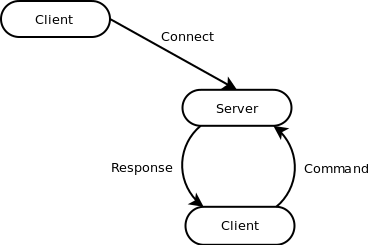
\includegraphics[scale=0.65]{chapter2/diagrams/protocol_high_level.png}
        \caption{The exchange of messages between a client and the server}
        \label{highLevelDia}
    \end{center}
\end{figure}

Gim uses a client-server architecture, where one computer (known as the Sever) acts as a central point which other computers (the Clients) connect. The clients do no communicate directly with each other and all communication takes place between the clients and the server. If a client wishes to send a message to another client it must first got through the server.

In GIM, the Protocol is responsible for enabling communication between the clients and the server in a reliable and consistent manner. A protocol is a set of rules that determine the format and transmission of data between computers. The syntax (the structure, or format) and semantics (the meaning) of the Protocol are discussed in the next section.

At the highest level of abstraction, the GIM Protocol works in a very simple manner.  A client connects to the sever and they exchange messages until the connection is closed, as shown in Figure ~\ref{highLevelDia}.

In practice there are several clients connected to the server at once, however as the clients do not directly interact with each other and do not need to know about each other, the entire system can be simplified as described above.



\subsection{Protocol Specification}

\subsection{Protocol Evolution}


\section{Client}

\subsection{Overview}

This section will analyse how appropriate our client design was to achieve the aims outlined in the client section\footnote{See section x.y for a detailed discussion}. Some of our design choices worked well, such as the interfaces used by the controller to separate concerns. Another decision that worked well was our use of the object oriented features of Java to implement chat windows, which reduced the challenge of routing internal messages to the correct windows. These aspects will be discussed in the `Design Changes' section.

While implementing the client, it became clear that some of our larger design choices were naive, and further design work had to be conducted. One case involved the interaction between the controller and networking subsystem. These changes will be discussed in the `Design Changes' section. In some cases, smaller design choices required larger changes. Of particular significance, our understanding of the practical working of the GIM protocol to create personal chats proved to be weak. This required design work reaching over the protocol and the model component of the system. This process tested our ability to collaborate as a team to implement an interacting system. The degree of success of our changes will be discussed in the 'Collaboration' section. Furthermore, as we became more familiar with the Java Swing environment, our code went through evolutionary steps to implement certain features in a more sensible manner, such as how displaying updates to user information was handled. The 'Evolution of Code' section will discuss problems we identified with code that was functional but deemed to be hard to maintain, and the merits of the changes we made, such as in the above case. 

\subsection{Design Changes}



\subsection{Collaboration}

The first draft of the GIM protocol treated all conversations as `rooms' and did not distinguish group chats and personal chats\footnote{internal reference to protocol section}. In designing the protocol, we wished to keep it abstract and not fall into the trap of implicitly implementing features that the client and server could handle. Our goal was not to develop a protocol suitable for only one type of implementation. Originally, it was believed that the client could distinguish personal chats and group chats by storing internal records of the type of outgoing invites to chat. In the case of being invited to chat, we believed using the protocol's ``USER'' argument in the ``::ROOM::'' command would be sufficient to count the amount of users in the room and determine the type of chat. However, as we began implementing room creation, it became clear that the initial group user list could be of size 1, and thus the wrong chat window could be created. As a result, the protocol had to be changed, and the client amended to reflect these changes. 

This change was a test of the boundary of responsibilities within our system, as it effected communication with the server and the back end of the client. The protocol engineer's solution to the issue was to add a `type' argument to the room command. In the case creating a room, the type now had to be specified. To allow a user to work out what room type a chat had, the `type' argument would be used, with a room identifier. This kept the protocol more abstract. In order to deal with these changes, our client had to be designed to sequence responses from the server for certain requests. As the protocol did not include sequence numbers, we had to re-design the model to perform this task. It was apparent that the amount of ``talk'' between the client and server required to start a chat was now increased. This required an understanding of what needed to be stored at each stage. This high level plan was determined:

Creation:
\begin{enumerate}
\item Client adds the type of room to be created to the new room queue in the model.
\item Client notes a list of user(s) invited to chat in the invitations queue in the model.
\item Client sends request to server to create a room of this type.
\item Server responds with `created' and the room id.
\item Client matches the type of chat with the `new room' queue, and the user list from the `invitations' queue.
\item Client spawns the appropriate chat window, or updates the internal state information of an existing window with the new roomid in the window list. Information includes who is in the room and the id to send messages to.
\item The client is informed that the participant has joined the room.
\end

Invitation:
\begin{enumerate}
\item Client receives invite to chat from server with certain room id from user. Store username in an ``invited'' queue in model.  
\item Client asks server the type of the room that it has been invited to.
\item Server responds with `Personal' or `Group.'
\item Client matches request with response from the ``invited'' queue.
\item Client spawns the appropriate chat window, or updates the internal state information of an existing window with the new roomid in the window list. Information includes who is in the room and the id to send messages to.
\item Client is informed that the participant has joined the room.
\item If it is a group chat, client asks server for the user list in the room.
\end{enumerate}

In retrospect, the trade off between keeping an abstract protocol (which could be used for different styles of implementation) and designing towards our own client and server may have been too high. Aside from the communication between the client and the server, there are complexities within the client code to ensure these events are performed in sequence which left much opportunity for error in the control of threading. For example, a user should not be allowed to send a message before the conversation participant has also joined the room, in the case of a personal chat between steps 6 and 7. This meant that safeguards had to be considered during this sequence of events to ensure messages were not dropped, while ensuring the user did not have to `wait' for the other user to enter the room before entering a message. This motivated the need for a boolean value (internal to chat windows) indicating whether the chat participant was in the room. While this value is false, messages to be sent are buffered until it turns true. A further issue of synchronization was internal to the code. Since the GUI was running on a separate thread from the incoming networking thread, it was conceivable that an incoming message could occur before the internal room id was updated in step 6. In fact, this issue was subtle enough that it was not recognised until late in development. In retrospect, part of our problem was from not identifying where the Swing event queue needed to be used (as outlined in the previous section), as well as the complex set of events that needed to occur to establish a chat. Throughout this project, we became more aware of the careful approach required when using threads.

\subsection{Evolution of Code}


\section{Server}

This section will analyse how well the server implementation fulfils the design outlined in section \ref{ServerDesign}. In general, the implementation of the server was a straight-forward affair with very few problems encountered during its development. The most challenging part of the server's development related to concurrency, and is discussed in section \ref{concur}. Spelling errors and typos were the most common cause of problems, however given their easy-to-fix nature, they are not discussed.

\subsection{Concurrency}
\label{concur}
Concurrency was the biggest concern while implementing the server and it was very important that we got it right. Concurrency problems such as race conditions are generally considered to be one of the most difficult problems to debug, so great care was taken to ensure that the possibility of these problems was kept as low as possible. Although we discovered some problems with threading (discussed in section \ref{server_eval}), none of the bugs were caused by race conditions. Instead, confusion about how threads work conceptually caused most of the threading related bugs. For example, in one case an attempt to kill another thread actually caused the current thread to commit suicide. The following describes how thread safety was dealt with and the lessons we learned.

Originally the server used the HashMap class from the \texttt{java.util} package very extensively, primarily because of its very quick look-up times and ability to use user IDs (Strings) as keys. Each User has five HashMaps to store data: their friends, which users have them as a friend, friend requests, blocked users, and rooms they are currently in. Each room uses one to store current users and another to store invited users. The global Data class uses another three to store all of the rooms, users, and workers on the server. This was an issue because HashMaps are not thread-safe, which means each of them had to be wrapped in a synchronised block to ensure thread safety. This was very tedious and very prone to human error. Later on in the development of the server we discovered the \texttt{java.util.concurrent} package, which contains thread-safe implementations of some of the classes in the \texttt{java.util} package, including a thread-safe version of the HashMap class called ConcurrentHashMap. By using the ConcurrentHashMap, it allowed us to remove a lot of the boilerplate code used to make the original implementation thread-safe, and made working with the HashMaps much safer and less prone to human error.

The Buffer class implements a thread-safe, unbounded blocking queue. Essentially the buffer is a LinkedList made thread-safe by only allowing items to be added and removed through synchronised methods. This ensured that at no point could more than one operation be performed on the list, preventing race conditions from occurring.

One of the most difficult to find bugs occurred when a user attempted to log in from 2 different clients. The server located the the worker which was allocated to the client already logged, placed an \texttt{:ERROR:} and \texttt{:QUIT} commands into their buffer, and then set the users worker to the worker of the new client. The new client then mysteriously disconnected. We eventually realised that by putting the \texttt{:QUIT:} command into the workers buffer it was not immediately being disconnected, there would be a slight delay between placing the command into buffer and the command being executed. The \texttt{:QUIT:} command logs out the user and then kills their client. As we had already set the user's worker to the one associated with the new client we were effectively killing both the old and new workers. This was something we had not considered when designing the server. Fortunately the solution was fairly simple and did not require any sizeable changes to the structure of the server. We forced the new worker to wait until the old worker had died, and therefore has empted its buffer and logged the user out, meaning that it was now safe to assign the new worker to the user and log them in.

\subsection{Detecting Abuse and Enforcing Limits}
Originally the server did not enforce any of the limits defined in the protocol and these had to be introduced at a later on in development. As we were aware from the start of development that they would need to be implemented in the future, we were able to design the server so that they could easily be added. 

Limiting the number of commands in moving window turned out to be an interesting problem to solve efficiently.

\begin{verbatim}
this.lastCommandTime = System.currentTimeMillis();
long oldest = this.commandTimes[this.last];

if (oldest != 0 && oldest > (this.lastCommandTime - 5000))
    killWorker();

this.commandTimes[last] = this.lastCommandTime;
this.last = (this.last + 1) % (this.commandTimes.length - 1);
\end{verbatim}


		


\section{Networking Design}

\subsection{Client Networking Structure}

We determined the role of the client networking component to be to maintain a connection with the server, read commands from the command buffer and pass them to the server, and pass commands from the server to the client. These two concerns came with different challenges; where keeping a connection with the server involved considering how to manage writing and reading data to the socket while allowing the client to run efficiently, and sending and receiving commands involved considering how best to parse data coming from the socket, and pass data between components.

\subsubsection {Maintaining a Connection}

The connection to the server had to be designed such that our program could freely write to the socket, and receive commands without having to worry about networking concurrency. For example, the client should not have to worry about doing multiple (possibly simultaneous if there is any multithreaded aspects of its operations) writes to the server, and waiting for these actions to complete. With these considerations in mind, we had to design our component to manage the connection so that the socket would not be written to while a read or write was in progress, while accomodating multiple requests. We had to implement this management in a way that these operations would be hidden from the client. 

Writing to the network was handled by a thread that monitors the buffer for any commands to send to the server. Crucially, commands can accumulate in this buffer, so that the client does not have to wait till a command has completed sending to the socket to continue its operations. As the methods in the buffer are synchronised, it could be ensured that data would remain in a consistent state, and that commands would be sent sequentially. This is of particular importance, as the the networking code would use this buffer to write to the server in order to implement the protocol's 'stay-alive' feature (as discussed in the protocol design section.)  

Reading from the network was handled by designing a class which we named 'NetworkReader.' This class would be run on a thread, and listen to the socket connection for incoming commands. When a command was received, it would then place it onto the intermediate command buffer to be handled by the controller thread (as discussed in section 2.2.4.) The methods within the buffer class would be designed with threading in mind, so that it would remain in a consistent state. A further role of the network reader class would be to inform the client that the connection to the server had been broken, and that action needed to be taken to inform the user and reset any internal information.

\subsubsection {Command Handling }

The parsing of commands was a broad concern that effected both the server and client's activities. This motivated the need to design a 'Command' class which could be used to parse commands. As described in the protocol design section, the GIM protocol follows a structured approach which for each command it is possible to identify the command, argument, and data segments associated with a command. The role of the command class would be to provide facilities that would take a line read from incoming socket data, and create an object from which the individual segements of the command may be extracted. An additional responsibility of this class would be to convert images to and from base64 encoding for transmission over the network (as required by the GIM protocol.)

We thought this was a sensible design decision as it provided a layer of abstraction which allowed the structure of the GIM protocol to change, or additional commands to be added, while only having to change the command class to handle this change. This lead to the design of a 'util' package, as part of our project's structure, while included classes common to both the client and the server networking code. 

On creation of this command object by the 'NetworkReader' class, it would be handed to the command buffer for retrieval and further parsing by the controller, and then translation into a method call. In addition to promoting code re-use, this approach had the advantage of hiding the structure of the GIM protocol from the client, which increased the degree of modularity in the system.   



















\section{Summary}
Getting the design of a system correct is the most important and difficult part of a computing science project. We spent a fair amount of time on it, making sure we understand what's going on before we started coding. As expected, we didn't get everything right the first time. In the next chapter, the implementation of these designs will be discussed, and the problems we encountered with the design during coding.


\chapter{Implementation}
\label{implementation}

%Introductory paragraph

\section{Client}

\subsection{Overview}

This section will analyse how appropriate our client design was to achieve the aims outlined in the client section\footnote{See section x.y for a detailed discussion}. Some of our design choices worked well, such as the interfaces used by the controller to separate concerns. Another decision that worked well was our use of the object oriented features of Java to implement chat windows, which reduced the challenge of routing internal messages to the correct windows. These aspects will be discussed in the `Design Changes' section.

While implementing the client, it became clear that some of our larger design choices were naive, and further design work had to be conducted. One case involved the interaction between the controller and networking subsystem. These changes will be discussed in the `Design Changes' section. In some cases, smaller design choices required larger changes. Of particular significance, our understanding of the practical working of the GIM protocol to create personal chats proved to be weak. This required design work reaching over the protocol and the model component of the system. This process tested our ability to collaborate as a team to implement an interacting system. The degree of success of our changes will be discussed in the 'Collaboration' section. Furthermore, as we became more familiar with the Java Swing environment, our code went through evolutionary steps to implement certain features in a more sensible manner, such as how displaying updates to user information was handled. The 'Evolution of Code' section will discuss problems we identified with code that was functional but deemed to be hard to maintain, and the merits of the changes we made, such as in the above case. 

\subsection{Design Changes}



\subsection{Collaboration}

The first draft of the GIM protocol treated all conversations as `rooms' and did not distinguish group chats and personal chats\footnote{internal reference to protocol section}. In designing the protocol, we wished to keep it abstract and not fall into the trap of implicitly implementing features that the client and server could handle. Our goal was not to develop a protocol suitable for only one type of implementation. Originally, it was believed that the client could distinguish personal chats and group chats by storing internal records of the type of outgoing invites to chat. In the case of being invited to chat, we believed using the protocol's ``USER'' argument in the ``::ROOM::'' command would be sufficient to count the amount of users in the room and determine the type of chat. However, as we began implementing room creation, it became clear that the initial group user list could be of size 1, and thus the wrong chat window could be created. As a result, the protocol had to be changed, and the client amended to reflect these changes. 

This change was a test of the boundary of responsibilities within our system, as it effected communication with the server and the back end of the client. The protocol engineer's solution to the issue was to add a `type' argument to the room command. In the case creating a room, the type now had to be specified. To allow a user to work out what room type a chat had, the `type' argument would be used, with a room identifier. This kept the protocol more abstract. In order to deal with these changes, our client had to be designed to sequence responses from the server for certain requests. As the protocol did not include sequence numbers, we had to re-design the model to perform this task. It was apparent that the amount of ``talk'' between the client and server required to start a chat was now increased. This required an understanding of what needed to be stored at each stage. This high level plan was determined:

Creation:
\begin{enumerate}
\item Client adds the type of room to be created to the new room queue in the model.
\item Client notes a list of user(s) invited to chat in the invitations queue in the model.
\item Client sends request to server to create a room of this type.
\item Server responds with `created' and the room id.
\item Client matches the type of chat with the `new room' queue, and the user list from the `invitations' queue.
\item Client spawns the appropriate chat window, or updates the internal state information of an existing window with the new roomid in the window list. Information includes who is in the room and the id to send messages to.
\item The client is informed that the participant has joined the room.
\end

Invitation:
\begin{enumerate}
\item Client receives invite to chat from server with certain room id from user. Store username in an ``invited'' queue in model.  
\item Client asks server the type of the room that it has been invited to.
\item Server responds with `Personal' or `Group.'
\item Client matches request with response from the ``invited'' queue.
\item Client spawns the appropriate chat window, or updates the internal state information of an existing window with the new roomid in the window list. Information includes who is in the room and the id to send messages to.
\item Client is informed that the participant has joined the room.
\item If it is a group chat, client asks server for the user list in the room.
\end{enumerate}

In retrospect, the trade off between keeping an abstract protocol (which could be used for different styles of implementation) and designing towards our own client and server may have been too high. Aside from the communication between the client and the server, there are complexities within the client code to ensure these events are performed in sequence which left much opportunity for error in the control of threading. For example, a user should not be allowed to send a message before the conversation participant has also joined the room, in the case of a personal chat between steps 6 and 7. This meant that safeguards had to be considered during this sequence of events to ensure messages were not dropped, while ensuring the user did not have to `wait' for the other user to enter the room before entering a message. This motivated the need for a boolean value (internal to chat windows) indicating whether the chat participant was in the room. While this value is false, messages to be sent are buffered until it turns true. A further issue of synchronization was internal to the code. Since the GUI was running on a separate thread from the incoming networking thread, it was conceivable that an incoming message could occur before the internal room id was updated in step 6. In fact, this issue was subtle enough that it was not recognised until late in development. In retrospect, part of our problem was from not identifying where the Swing event queue needed to be used (as outlined in the previous section), as well as the complex set of events that needed to occur to establish a chat. Throughout this project, we became more aware of the careful approach required when using threads.

\subsection{Evolution of Code}


\section{Server}

This section will analyse how well the server implementation fulfils the design outlined in section \ref{ServerDesign}. In general, the implementation of the server was a straight-forward affair with very few problems encountered during its development. The most challenging part of the server's development related to concurrency, and is discussed in section \ref{concur}. Spelling errors and typos were the most common cause of problems, however given their easy-to-fix nature, they are not discussed.

\subsection{Concurrency}
\label{concur}
Concurrency was the biggest concern while implementing the server and it was very important that we got it right. Concurrency problems such as race conditions are generally considered to be one of the most difficult problems to debug, so great care was taken to ensure that the possibility of these problems was kept as low as possible. Although we discovered some problems with threading (discussed in section \ref{server_eval}), none of the bugs were caused by race conditions. Instead, confusion about how threads work conceptually caused most of the threading related bugs. For example, in one case an attempt to kill another thread actually caused the current thread to commit suicide. The following describes how thread safety was dealt with and the lessons we learned.

Originally the server used the HashMap class from the \texttt{java.util} package very extensively, primarily because of its very quick look-up times and ability to use user IDs (Strings) as keys. Each User has five HashMaps to store data: their friends, which users have them as a friend, friend requests, blocked users, and rooms they are currently in. Each room uses one to store current users and another to store invited users. The global Data class uses another three to store all of the rooms, users, and workers on the server. This was an issue because HashMaps are not thread-safe, which means each of them had to be wrapped in a synchronised block to ensure thread safety. This was very tedious and very prone to human error. Later on in the development of the server we discovered the \texttt{java.util.concurrent} package, which contains thread-safe implementations of some of the classes in the \texttt{java.util} package, including a thread-safe version of the HashMap class called ConcurrentHashMap. By using the ConcurrentHashMap, it allowed us to remove a lot of the boilerplate code used to make the original implementation thread-safe, and made working with the HashMaps much safer and less prone to human error.

The Buffer class implements a thread-safe, unbounded blocking queue. Essentially the buffer is a LinkedList made thread-safe by only allowing items to be added and removed through synchronised methods. This ensured that at no point could more than one operation be performed on the list, preventing race conditions from occurring.

One of the most difficult to find bugs occurred when a user attempted to log in from 2 different clients. The server located the the worker which was allocated to the client already logged, placed an \texttt{:ERROR:} and \texttt{:QUIT} commands into their buffer, and then set the users worker to the worker of the new client. The new client then mysteriously disconnected. We eventually realised that by putting the \texttt{:QUIT:} command into the workers buffer it was not immediately being disconnected, there would be a slight delay between placing the command into buffer and the command being executed. The \texttt{:QUIT:} command logs out the user and then kills their client. As we had already set the user's worker to the one associated with the new client we were effectively killing both the old and new workers. This was something we had not considered when designing the server. Fortunately the solution was fairly simple and did not require any sizeable changes to the structure of the server. We forced the new worker to wait until the old worker had died, and therefore has empted its buffer and logged the user out, meaning that it was now safe to assign the new worker to the user and log them in.

\subsection{Detecting Abuse and Enforcing Limits}
Originally the server did not enforce any of the limits defined in the protocol and these had to be introduced at a later on in development. As we were aware from the start of development that they would need to be implemented in the future, we were able to design the server so that they could easily be added. 

Limiting the number of commands in moving window turned out to be an interesting problem to solve efficiently.

\begin{verbatim}
this.lastCommandTime = System.currentTimeMillis();
long oldest = this.commandTimes[this.last];

if (oldest != 0 && oldest > (this.lastCommandTime - 5000))
    killWorker();

this.commandTimes[last] = this.lastCommandTime;
this.last = (this.last + 1) % (this.commandTimes.length - 1);
\end{verbatim}


		


\section{Client-Server Communication}
blah blah blah


\section{Storage}
\label{storage}

Both the GIM client and server use Java's built-in serialization features to store data locally while they are not running. The Data class of the server and the Options class of the client both implement Serializable from \texttt{java.io}. This allows them to be serialized and stored on disk using an ObjectOutputStream object (also in \texttt{java.io}).

When the client starts it reads this file from the disk and uses an ObjectInputStream to turn the raw data back into the Options object. For the server, it is not quite so simple. Although the server serializes the entire Data object, some of the data stored in it (such as as rooms) does not need to be persisted across sessions and we create a section Data object and copy the persistent data from the serialized object into it.



\chapter{Evaluation}
\label{evaluation}

\section{Scope}

This section will discuss how we evaluated that our system was functioning according to our requirements. Because our project had a focus on technical issues, we did not conduct any formal usability evaluations with potential users. We did not conduct any formal user evaluations as the would only serve to gather data about the usability of our interface, which given time constraints, was not a huge priority. However, we did conduct many informal testing sessions under normal conditions (with many users logged on), to get some feedback about our interface and features, in addition to testing our system - but we did not collect any data on such feedback. 

Instead, our evaluations were more focused on ensuring our system complied to the specifications we have drawn out in section \ref{features}. As our system is modular, we decided a sensible boundary for our test harnesses would be around the client and the server. Our goal in testing was focused on ensuring the client and server performed their roles as outlined in the GIM protocol, and to attempt to ensure that our our threading was robust.  These aspects, and an analysis of our testing methods, will be outlined in sections \ref{server_eval} and \ref{client_eval}. Much of our testing was conducted using volunteers who used the client from its earliest versions, to later versions. Testing with users naturally allowed us to test threading issues, as when many users are logged there is a greater degree of synchronization. The server receives commands from more users simultaneously, and the client receives more commands from the server about events it needs to know about.


\section{Server}

This section will analyse how well the server implementation fulfils the design outlined in section \ref{ServerDesign}. In general, the implementation of the server was a straight-forward affair with very few problems encountered during its development. The most challenging part of the server's development related to concurrency, and is discussed in section \ref{concur}. Spelling errors and typos were the most common cause of problems, however given their easy-to-fix nature, they are not discussed.

\subsection{Concurrency}
\label{concur}
Concurrency was the biggest concern while implementing the server and it was very important that we got it right. Concurrency problems such as race conditions are generally considered to be one of the most difficult problems to debug, so great care was taken to ensure that the possibility of these problems was kept as low as possible. Although we discovered some problems with threading (discussed in section \ref{server_eval}), none of the bugs were caused by race conditions. Instead, confusion about how threads work conceptually caused most of the threading related bugs. For example, in one case an attempt to kill another thread actually caused the current thread to commit suicide. The following describes how thread safety was dealt with and the lessons we learned.

Originally the server used the HashMap class from the \texttt{java.util} package very extensively, primarily because of its very quick look-up times and ability to use user IDs (Strings) as keys. Each User has five HashMaps to store data: their friends, which users have them as a friend, friend requests, blocked users, and rooms they are currently in. Each room uses one to store current users and another to store invited users. The global Data class uses another three to store all of the rooms, users, and workers on the server. This was an issue because HashMaps are not thread-safe, which means each of them had to be wrapped in a synchronised block to ensure thread safety. This was very tedious and very prone to human error. Later on in the development of the server we discovered the \texttt{java.util.concurrent} package, which contains thread-safe implementations of some of the classes in the \texttt{java.util} package, including a thread-safe version of the HashMap class called ConcurrentHashMap. By using the ConcurrentHashMap, it allowed us to remove a lot of the boilerplate code used to make the original implementation thread-safe, and made working with the HashMaps much safer and less prone to human error.

The Buffer class implements a thread-safe, unbounded blocking queue. Essentially the buffer is a LinkedList made thread-safe by only allowing items to be added and removed through synchronised methods. This ensured that at no point could more than one operation be performed on the list, preventing race conditions from occurring.

One of the most difficult to find bugs occurred when a user attempted to log in from 2 different clients. The server located the the worker which was allocated to the client already logged, placed an \texttt{:ERROR:} and \texttt{:QUIT} commands into their buffer, and then set the users worker to the worker of the new client. The new client then mysteriously disconnected. We eventually realised that by putting the \texttt{:QUIT:} command into the workers buffer it was not immediately being disconnected, there would be a slight delay between placing the command into buffer and the command being executed. The \texttt{:QUIT:} command logs out the user and then kills their client. As we had already set the user's worker to the one associated with the new client we were effectively killing both the old and new workers. This was something we had not considered when designing the server. Fortunately the solution was fairly simple and did not require any sizeable changes to the structure of the server. We forced the new worker to wait until the old worker had died, and therefore has empted its buffer and logged the user out, meaning that it was now safe to assign the new worker to the user and log them in.

\subsection{Detecting Abuse and Enforcing Limits}
Originally the server did not enforce any of the limits defined in the protocol and these had to be introduced at a later on in development. As we were aware from the start of development that they would need to be implemented in the future, we were able to design the server so that they could easily be added. 

Limiting the number of commands in moving window turned out to be an interesting problem to solve efficiently.

\begin{verbatim}
this.lastCommandTime = System.currentTimeMillis();
long oldest = this.commandTimes[this.last];

if (oldest != 0 && oldest > (this.lastCommandTime - 5000))
    killWorker();

this.commandTimes[last] = this.lastCommandTime;
this.last = (this.last + 1) % (this.commandTimes.length - 1);
\end{verbatim}


		


\section{Client}

\subsection{Overview}

This section will analyse how appropriate our client design was to achieve the aims outlined in the client section\footnote{See section x.y for a detailed discussion}. Some of our design choices worked well, such as the interfaces used by the controller to separate concerns. Another decision that worked well was our use of the object oriented features of Java to implement chat windows, which reduced the challenge of routing internal messages to the correct windows. These aspects will be discussed in the `Design Changes' section.

While implementing the client, it became clear that some of our larger design choices were naive, and further design work had to be conducted. One case involved the interaction between the controller and networking subsystem. These changes will be discussed in the `Design Changes' section. In some cases, smaller design choices required larger changes. Of particular significance, our understanding of the practical working of the GIM protocol to create personal chats proved to be weak. This required design work reaching over the protocol and the model component of the system. This process tested our ability to collaborate as a team to implement an interacting system. The degree of success of our changes will be discussed in the 'Collaboration' section. Furthermore, as we became more familiar with the Java Swing environment, our code went through evolutionary steps to implement certain features in a more sensible manner, such as how displaying updates to user information was handled. The 'Evolution of Code' section will discuss problems we identified with code that was functional but deemed to be hard to maintain, and the merits of the changes we made, such as in the above case. 

\subsection{Design Changes}



\subsection{Collaboration}

The first draft of the GIM protocol treated all conversations as `rooms' and did not distinguish group chats and personal chats\footnote{internal reference to protocol section}. In designing the protocol, we wished to keep it abstract and not fall into the trap of implicitly implementing features that the client and server could handle. Our goal was not to develop a protocol suitable for only one type of implementation. Originally, it was believed that the client could distinguish personal chats and group chats by storing internal records of the type of outgoing invites to chat. In the case of being invited to chat, we believed using the protocol's ``USER'' argument in the ``::ROOM::'' command would be sufficient to count the amount of users in the room and determine the type of chat. However, as we began implementing room creation, it became clear that the initial group user list could be of size 1, and thus the wrong chat window could be created. As a result, the protocol had to be changed, and the client amended to reflect these changes. 

This change was a test of the boundary of responsibilities within our system, as it effected communication with the server and the back end of the client. The protocol engineer's solution to the issue was to add a `type' argument to the room command. In the case creating a room, the type now had to be specified. To allow a user to work out what room type a chat had, the `type' argument would be used, with a room identifier. This kept the protocol more abstract. In order to deal with these changes, our client had to be designed to sequence responses from the server for certain requests. As the protocol did not include sequence numbers, we had to re-design the model to perform this task. It was apparent that the amount of ``talk'' between the client and server required to start a chat was now increased. This required an understanding of what needed to be stored at each stage. This high level plan was determined:

Creation:
\begin{enumerate}
\item Client adds the type of room to be created to the new room queue in the model.
\item Client notes a list of user(s) invited to chat in the invitations queue in the model.
\item Client sends request to server to create a room of this type.
\item Server responds with `created' and the room id.
\item Client matches the type of chat with the `new room' queue, and the user list from the `invitations' queue.
\item Client spawns the appropriate chat window, or updates the internal state information of an existing window with the new roomid in the window list. Information includes who is in the room and the id to send messages to.
\item The client is informed that the participant has joined the room.
\end

Invitation:
\begin{enumerate}
\item Client receives invite to chat from server with certain room id from user. Store username in an ``invited'' queue in model.  
\item Client asks server the type of the room that it has been invited to.
\item Server responds with `Personal' or `Group.'
\item Client matches request with response from the ``invited'' queue.
\item Client spawns the appropriate chat window, or updates the internal state information of an existing window with the new roomid in the window list. Information includes who is in the room and the id to send messages to.
\item Client is informed that the participant has joined the room.
\item If it is a group chat, client asks server for the user list in the room.
\end{enumerate}

In retrospect, the trade off between keeping an abstract protocol (which could be used for different styles of implementation) and designing towards our own client and server may have been too high. Aside from the communication between the client and the server, there are complexities within the client code to ensure these events are performed in sequence which left much opportunity for error in the control of threading. For example, a user should not be allowed to send a message before the conversation participant has also joined the room, in the case of a personal chat between steps 6 and 7. This meant that safeguards had to be considered during this sequence of events to ensure messages were not dropped, while ensuring the user did not have to `wait' for the other user to enter the room before entering a message. This motivated the need for a boolean value (internal to chat windows) indicating whether the chat participant was in the room. While this value is false, messages to be sent are buffered until it turns true. A further issue of synchronization was internal to the code. Since the GUI was running on a separate thread from the incoming networking thread, it was conceivable that an incoming message could occur before the internal room id was updated in step 6. In fact, this issue was subtle enough that it was not recognised until late in development. In retrospect, part of our problem was from not identifying where the Swing event queue needed to be used (as outlined in the previous section), as well as the complex set of events that needed to occur to establish a chat. Throughout this project, we became more aware of the careful approach required when using threads.

\subsection{Evolution of Code}



\section{Summary}




\appendix
\chapter{GIM Protocol Specification}
\label{protocol_spec}
\section{Introduction}

A network protocol is a set of rules which must be followed for a program to produce the desired effect on another machine in a network based system. The motivation behind creating a protocol is to allow a standard pattern of communication to be devised for a given system. This allows a system following the protocol to consistently perform the same role, in any context, regardless of its implementation. Any command in our protocol should produce a verifiable result as outlined in this section.

To guarantee any desired outcome, a `message' must be well formed (follow the correct syntax), be sent while the machine is in a valid `state,' and be sent within any expected time frame. This document outlines these aspects of our protocol in detail - specifying any constraint on when an action may be undertaken, and any constraint on the time allowed for this action to be performed. The outcome on the system state will also be detailed. Both aspects can be identified by the pre-conditions and post-conditions surrounding any given command.

In our framework, there is one machine that undertakes a `server' role, and many machines that can undertake a `client' role. These roles govern what a machine may validly send or receive, depending on its role. A general a pattern of communication, such that one role sending a `message' to the other results in a reply from this role, and a possible change of `state' in each member, will be evidenced in this section. To better understand our protocol, it is necessary to outline the function of these roles, with some reference to the states they maintain, to illuminate the utility of available messages.

At a high level, the role of the server is to keep a record of state persistent aspects of the user's account; composed of details such as login details, a buddy list, and privacy conditions. Further, it holds volatile state information, relevant only to a session (which can be defined as a state where the user is logged in). It monitors the global state of the system and relays information such as which buddies are available to message, and their state. Its pivotal role is to relay messages between clients. 

The role of the client is to allow the user to retrieve, via an interface, information regarding their buddies, and to send messages to the server which will subsequently be relayed to their buddies. Furthermore, it allows the user to modify their state within the system via the server.

\section{Commands}

\subsection{Command Structure}

Each message will follow this high level syntax: \\
\texttt{:COMMAND [ ARG1 \ \vline \ ARG2 \ \vline \ ARG3 ]: $<$data$>$;}

\begin{itemize}

\item{Square brackets [ ... ] denote a list of 1 or more arguments of which only one can be given and is required.}  

\item{Curly brackets \{ ... \} are used to represent arguments which are optional and can be non-singular.}

\item{A colon is used in the first instance to indicate the opening of a command, and in the second to indicate the boundary between a command's arguments and the data set.}

\item{Angular brackets $<$ … $>$ are used to show data that has been provided by the user and should be considered unsafe.}

\item{A semi colon ; is used to show the end of a command.}

\end{itemize}

By example:
\texttt{:GET \{ NICKNAME \ \vline \ STATUS \ \vline \ PERSONAL\_MESSAGE \ \vline \ DISPLAY\_PIC \}: $<$user$>$ $<$user$>$...;}\\
Could be used as follows: \\
\texttt{:GET NICKNAME STATUS PERSONAL\_MESSAGE: cyblob@idgmail.com meow@hotmail.com;} \\
Which means request the Nickname, Status and Personal Message of users cyblob@gmail.com and meow@hotmail.com.

Remarkably, this minimalistic structure is suitable to fulfill every requirement of the system and promote readability.

Every command or request which the sever receives must be followed by a response of some type. Where there is a command which does not return any data, the server should respond with the \texttt{:OKAY:} command to signal that the command was received and error free.

Commands have a maximum length of 8192 characters, including any punctuation, with the exception of the \texttt{:SET DISPLAY\_PIC:} command, which has a character limit of 32768.

\subsection{Heart Beat}

In order for the server to recognise that the client is still functioning, it must receive a command from the client on a regular basis (around every 15 seconds). In the event that no command is received for an extended period, the server will disconnect the client.

Any command will reset the timeout, however it is recommended that the \texttt{:PING:} command is used.

\section{Pre-login Commands}

These are the only commands possible before a user has logged in, and remain possible after the user has logged in.

These include all commands necessary for establishing a connection, logging into the server, and creating a new account.

\subsection{Server Commands}
\label{servercomm}

\texttt{:PING:;}

The command is used as a keep-alive command. Its primary use is to indicate that the client is still alive even if no other communication has been received from the client. 

Examples:
\texttt{:PING: ;} \\
The client responding to a \texttt{:PING:} command

{\bf :SERVERSTATUS \{ USERS \ \vline \ TIME \ \vline \ UPTIME \}:;}

The \texttt{:SERVERSTATUS:} command returns information about the server including the number of users, the local system time, and server up-time.
 
In the case that an argument is provided, the server should then return a \texttt{:SERVERSTATUS:} as defined in the client section. If more than one argument is provided, then the server should return each value on a new line in the order which the arguments were received (reading from left to right).

The arguments for this command are as follows:

\begin{itemize}

\item{ \texttt{USERS} \\
The total number of users and number of online users}

\item{ \texttt{TIME} \\
The current local time of the server}

\item{ \texttt{UPTIME} \\
The up-time of the server instance}

\end{itemize}

Examples:
\texttt{:SERVERSTATUS USERS:;} \\
Response$>$:\texttt{SERVERSTATUS USERS: 23 Online, 565 Total} \\
\texttt{:SERVERSTATUS TIME:;} \\
Response$>$:\texttt{SERVERSTATUS TIME: Wed 17 Nov, 23:31} \\

{\bf :AUTH \{ LOGIN \ \vline \ REGISTER \}: $<$email address$>$ $<$password$>$;}

The \texttt{:AUTH:} command deals with all aspects of user authorisation and permissions. The \texttt{:AUTH:} command alone should return the user's current authorisation state, either \texttt{LOGGEDIN} or \texttt{UNAUTHORIZED}.

{\bf LOGIN}

If the details are valid then the server should respond with an \texttt{:AUTH LOGGEDIN:} command. It should set the user's state (but not status) to \texttt{ONLINE}.
In the event that an error occurs the server should generate one of the following \texttt{:ERROR:} statuses:

\texttt{USER\_DOES\_NOT\_EXIST}\\
The email address has not been registered \\
\texttt{LOGIN\_DETAILS\_INCORRECT} \\
The password was incorrect \\
\texttt{MISSING\_ARGUMENTS} \\
There were too few arguments \\

If the user is already logged in then the server should send a \texttt{LOGGED\_IN\_FROM\_OTHER\_LOCATION} error and \texttt{KILL} command to the already connected user.

{\bf REGISTER}

The register argument allows for new users to be registered by providing a valid email address and password. If the new account is registered correctly then the server should respond with \texttt{:AUTH REGISTERED:}. However, it should not log the user in.

If the registration is unsuccessful the server should return one of the following \texttt{:ERROR:} messages:

\begin{itemize}

\item{\texttt{INVALID\_EMAIL} \\
The email address was invalid}

\item{\texttt{EMAIL\_ALREADY\_IN\_USE} \\
The email address has already been registered}

\item{\texttt{PASSWORD\_TOO\_SHORT} \\
The password is too short}

\item{\texttt{MISSING\_ARGUMENTS}	\\
There were too few arguments}

\end{itemize}

Examples:
\texttt{:AUTH REGISTER: cyblob@gmail.com p455w0rd;} \\
\texttt{:AUTH REGISTER: blah lol;} \\
Server responds \texttt{:ERROR INVALID\_EMAIL:} \\
\texttt{:AUTH LOGIN: cyblob@gmail.com p455w0rd;}\\
Server responds \texttt{:AUTH OKAY:} \\

{\bf :QUIT:;}

The \texttt{:QUIT:} command tells the server that the user wishes to log out (if applicable) and disconnect from the server. Once the quit command has been received, the user's state should be changed to \texttt{OFFLINE} and the connection broken.

Examples:
\texttt{:QUIT:;} \\
User is logged out and disconnected.

\subsection{Client Commands}

{\bf :OKAY:;}

In the event that a command received from the client does not have any other response, the \texttt{:OKAY:} command is sent to signify that the command was successful.

Examples:
\texttt{:OKAY:;}\\
The last command executed okay.

{\bf :SERVERSTATUS \{ USERS \ \vline \ TIME \ \vline \ UPTIME \}:;}

If requested by the client, the server may send data about the server status, as defined in section \ref{servercomm}. If more than one argument is provided then the data is returned with each segment on its own line, in the same order which the arguments appeared. If no arguments are provided then the data can be in any format containing any information. This command should not be assumed to have a consistent format.

Example:
\texttt{:SERVERSTATUS TIME: Wed 17 Nov, 23:31;} \\
\texttt{:SERVERSTATUS USERS: 56 Online, 423 Total;} \\
\texttt{:SERVERSTATUS UPTIME: 21 days, 14:41;} \\

{\bf :KILL: $<$message$>$;}

In the event that the server wants the client to disconnect, it will issue a \texttt{:KILL:} command. As soon as the command has been sent the server will disconnect. 

Example:
\texttt{:KILL: Too many bad login attempts.;}\\
The server closes the connection.

{\bf :BROADCAST: $<$message$>$;}

A \texttt{:BROADCAST:} message sent by the server to all users. The broadcast message should be displayed immediately and is likely to contain critical information about the server.

Example:
\texttt{:BROADCAST: The server is on fire and about to crash. ;}

{\bf :AUTH [ LOGGEDIN \ \vline \ UNAUTHORIZED ]:;}

The \texttt{:AUTH:} command indicates to the client its current status. If the user is logged in then it will have the \texttt{LOGGEDIN} argument, otherwise it will have the \texttt{UNAUTHORISED} argument.

Example:
\texttt{:AUTH LOGGEDIN:;}\\
The user is logged in and has permissions to use post-login commands

\section{Post-login Commands}

These commands are accessible only once the user has logged in. The server should issue an \texttt{:ERROR UNAUTHORISED:} response if an unauthorised user attempts to use one of these commands. After repeated attempts, the server may temporarily block or ban the user.

\subsection{Server Commands}

{\bf :SET [ NICKNAME\ \vline \ STATUS \ \vline \ PERSONAL\_MESSAGE \ \vline \ DISPLAY\_PIC ]: $<$value$>$;}

The \texttt{:SET:} command allows various user attributes to be set by the client. The exact attribute depends on the argument given however only one attribute can be set at a time. In the case of \texttt{DISPLAY\_PIC}, the image is Base64 encoded.

Example:
\texttt{:SET NICKNAME: Andrew;} \\

{\bf :GET \{ NICKNAME\ \vline \ STATUS \ \vline \ PERSONAL\_MESSAGE \ \vline \ DISPLAY\_PIC \}: $<$user$>$\{$<$user$>$\};} \\

The \texttt{:GET:} command requests a set of attributes for each user in a space separated list of users. The server should respond with an \texttt{:INFO:} command and the appropriate data.

Example:
\texttt{:GET NICKNAME STATUS PERSONAL\_MESSAGE DISPLAY\_PIC: user1@host.com, user2@hotmail.com;}

{\bf :FRIENDLIST:;}

The \texttt{:FRIENDLIST:} command requests a list of users in the user's friend list. It should return a \texttt{:FREINDLIST:} command as specified in section \ref{clientcomm_post}.

Example: \\
\texttt{:FREINDLIST:} 
	
{\bf :ROOM [ CREATE \{GROUP\} \ \vline \ INVITE \ \vline \ JOIN \ \vline \ LEAVE \ \vline \ USERS \ \vline \ TYPE ]: \{$<$roomid$>$ \ \vline \ $<$user$>$\};}

The \texttt{:ROOM:} command deals with all room related requests.

\begin{itemize}

\item{CREATE \\
The \texttt{CREATE} argument specifies that the client wishes to create a new chat room for use. If the \texttt{GROUP} argument is not supplied then the room will be limited to a maximum of two participants and a userID must be supplied so that the server can invite the other user. Upon creation of the room, the user who created it is automatically placed in the room.}

\item {INVITE \\
The \texttt{INVITE} argument sends an invite to join the room to the specified user. They are then allowed to join the room at any point.}

\item{JOIN \\
The \texttt{JOIN} argument specifies that the user wishes to join the specified room. The must first have received an invite from someone already in the room.}

\item{LEAVE \\
The \texttt{LEAVE} argument specifies that the user wishes to leave the specified room.}

\item{USERS \\
The \texttt{USERS} argument requests a list of users in the room from the server, separated by spaces.}

\end{itemize}

\texttt{:MESSAGE: $<$roomid$>$ $<$message$>$;}

The \texttt{:MESSAGE:} command specifies a room and a message which should be delivered to the room.

Example: \\
\texttt{:MESSAGE: 25 Hey guys, what's up?;}

{\bf :FRIEND [ ADD \ \vline \ BLOCK \ \vline \ UNBLOCK \ \vline \ ACCEPT \ \vline \ DECLINE \ \vline \ DELETE ]: $<$target$>$;}

The \texttt{:FRIEND:} command controls all friend list data.

\begin{itemize}

\item{ADD \\
The \texttt{ADD} argument specifies that the client wishes to add the target user to their friend list. The server should then send a request to the target user asking for permission to access their data.}

\item{BLOCK \\
The \texttt{BLOCK} argument places the target user into a list of blocked users who cannot access any data about the current user.}

\item{UNBLOCK \\
The \texttt{UNBLOCK} argument removes the target from the current user's blocked list.}

\item{ACCEPT \\
The \texttt{ACCEPT} argument specifies that the user is responding to a previous friend request, where the target is the user who sent the request. If the user accepts, then the target user should be given permission to use the user's data.}

\item{DELETE \\
The \texttt{DELETE} argument specifies that the target user should be deleted from the users friend list. However, the target user will still have access to the user's details.}

\item{DECLINE \\
The \texttt{DECLINE} argument specifies that the user does not wish the target user to be to able to access their data.}

\end{itemize}

Example: \\
\texttt{:FRIEND ADD: cyblob@gmail.com;}	\\
Request access to cyblob@gmail.com's data

{\bf :LOGOUT:;}

The \texttt{:LOGOUT:} command specifies that the client wishes to logout but not drop the connection to the server.

Example: \\
\texttt{:LOGOUT:;}\\
The user is logged out

\subsection{Client Commands}
\label{clientcomm_post}

{\bf :MESSAGE: $<$roomid$>$ $<$sender$>$ $<$message$>$;}

The \texttt{:MESSAGE:} command represents a message received by the user. The sender is the email address of the person who sent the message, and the message is the message itself.

Example: \\
\texttt{:MESSAGE: 56 cyblob@gmail.com How's it going?;}

{\bf :ROOM [ CREATED \ \vline \ JOINED \ \vline \ LEFT \ \vline \ INVITED \ \vline \ USERS \ \vline \ PERSONAL \ \vline \ GROUP ]: $<$roomid$>$ \{$<$user$>$\};}

\begin{itemize}

\item{CREATED \\
The \texttt{CREATED} argument tells the client that their request to create a room was successful and specifies the room id.}

\item{JOINED \\
The \texttt{JOINED} argument tells the client that a new user has joined the room and specifies the room and id of the user who joined.}

\item{LEFT \\
The \texttt{LEFT} argument tells the client that a user has left the room and specifies the room and the id of the user who left.}

\item{INVITED \\
The \texttt{INVITED} argument tells the client that they have been invited to join a room. It specifies the room and the user who invited them.}

\item{USERS \\
The \texttt{USERS} argument provides a list of users (one per line) who are currently in the room.}

\item{PERSONAL \\
The \texttt{PERSONAL} argument tells the client that the room is a personal room (no more than two users).}

\item{GROUP \\
The \texttt{GROUP} argument tells the client that the room is a group room and any number of users can join.}
	
\end{itemize}

Example: \\
\texttt{:ROOM CREATED: 0;} \\
\texttt{:ROOM JOINED: 0 CYBLOB@GMAIL.COM;} \\
\texttt{:ROOM LEFT: 0 CYBLOB@GMAIL.COM;} \\
\texttt{:ROOM INVITED: 0 HAPPY0@GMAIL.COM;} \\
\texttt{:ROOM USERS: CYBLOB@GMAIL.COM HAPPY0@HOTMAIL.COM \\SOMEONEELSE@GMAAIL.COM ANOTHER@HOTMAIL.COM;} \\

{\bf :FRIENDLIST: ONLINE $<$user$>$ $<$user$>$... OFFLINE $<$user$>$ $<$user$>$... BLOCKED $<$user$>$ $<$user$>$...;}

The \texttt{:FRIENDLIST:} command specifies the user's friend list using the format specified above.

Example: \\
\texttt{:FREINDLIST: ONLINE cyblob@gmail.com blah@ddfdf.com OFFLINE meow@hotmail.com woof@gmail.com sheep@yahoo.com BLOCKED wtf@wtf.com;}

{\bf :FRIENDREQUEST: $<$user$>$ $<$nickname$>$;}

The \texttt{:FRIENDREQUEST:} command tells the client that the user has a friend request and specifies who sent it and their nickname at the time of sending. The client should then respond with the appropriate \texttt{:FRIEND:} command.

Example: \\
\texttt{:FRIENDREQUEST: cyblob@gmail.com James;}

{\bf :UPDATE [ NICKNAME\ \vline \ STATUS \ \vline \ PERSONAL\_MESSAGE \ \vline \ DISPLAY\_PIC \ \vline \ FRIENEDLIST  ]: $<$user$>$;}

The \texttt{:UPDATE:} command notifies the client that a user in their friend list has just updated one of their attributes. The client can then retrieve the updated attribute if necessary.

Example: \\
\texttt{:UPDATE NICKNAME: cyblob@gmail.com;}

\texttt{:INFO \{ NICKNAME \ \vline \ STATUS \ \vline \ PERSONAL\_MESSAGE \ \vline \ DISPLAY\_PIC \}: $<$user$>$ $<$data$>$ \{$<$user$>$ $<$data$>$\};} 

The data is returned one line per value, in the same order as the arguments given, separated by the user's email address. In the case of \texttt{DISPLAY\_PIC}, the image is Base64 encoded to enable it to be embedded as text.

Example: \\

\texttt{:INFO NICKNAME STATUS PERSONAL\_MESSAGE DISPLAY\_PIC: user1@host.com \\
James \\
Away \\
I’m a panda \\
/9j/4AAQSkZJRgABAQAAAQABAAD/2wBDAAYEBAQFBAYFBQYJBgUGCQsIBgYICwwKCgsK... \\
user2@host.com \\
Gordon \\
Online \\
I’m not a panda \\
DAREAAhEBAxEB/8QAHQAAAgIDAQEBAAAAAAAAAAAABAUDBgECBwAICf/EAE4QAAIBAg...;}

\texttt{:ERROR [ UNAUTHORISED \ \vline \ INVALID\_EMAIL \ \vline \ \\ EMAIL\_ALREADY\_IN\_USE \ \vline \ PASSWORD\_TOO\_SHORT \ \vline \ MISSING\_ARGUMENTS \ \vline \ \\ TOO\_MANY\_ARGUMENTS \ \vline \ INVALID\_ARGUMENT \ \vline \ LOGGED\_IN\_FROM\_OTHER\_LOCATION \ \vline \ \\ USER\_DOES\_NOT\_EXIST \ \vline \ LOGIN\_DETAILS\_INCORRECT ]: $<$message$>$;}

If an error occurs then the server should return one of these commands to the client. The exact command and the message will be specified by the sever.

Example: \\
\texttt{:ERROR INVALID\_EMAIL: No domain specified.;}


\chapter{Use Cases}
\section{Introduction}

This appendix contains all of the use cases that were documented during the design process. In many cases, the specifics of how these actions occur in GIM are different than the outlines here. The higher priority use cases were documented while those less likely to be implemented were not.

\section{Actors}

Two actors were identified for the system: ``Senders'' and ``Contacts.'' Both of these actors have equal privileges within the system and use the system in the same way, hence both derive from the ``User'' type.

\section{Must Have}

\subsection{Open application}

{\bf Actors}: User

User opens the application. They are prompted to either login or register. The user must choose File-$>$Quit from the menu at the top to exit, as the X will only minimize the program.

\subsection{Register}

{\bf Actors}: User

User chooses to register, and then enters their email, nickname, and password (same window). If no one with that email or nickname has registered yet, the user is successfully registered, and can now log in. There is an option to login automatically, and it will do so if selected. If it isn’t selected, they will be led back to the original screen (register or log-in).

\subsection{Log In}

{\bf Actors}: User

It is automatic, unless the option isn’t checked. Otherwise, the user either knows their login info or chooses to reset their password (via email). They enter their email and password into the fields. If it is not correct, they are prompted again. When logged in, anyone who has them as a friend is shown that they are online.

\subsection{Add contact}

{\bf Actors}: Sender, Contact

User clicks the ``add contact'' button in the main window, or the option from the top menu. They are prompted to enter their friend’s email. They enter the email and the system searches for that person in the database. If found, the contact is sent a request for friendship. If the contact accepts, then both the user and contact now have each other as contacts, and they show up in the main window. If not accepted, neither is added. If the contact is not found, they are prompted again to enter the email, with the option to cancel.

\subsection{Remove contact}

{\bf Actors}: User

User single-clicks the contact in their list that they want to remove and then presses the “remove contact” button in the main window (This can also be done from the top menu). This button will be grayed out until the user clicks a contact. A dialog box will pop up to confirm that they want to remove that person as a contact. There is also an option to block the contact. The contact will not have the user removed from their contact list.

\subsection{Chat/Send/Receive Messages}

{\bf Actors}: Sender, Contact

Four ways to begin a chat: selecting a contact and pressing the ``Enter'' key, double clicking a contact, right clicking a contact and selecting ``Chat'', and selecting a contact then pressing a chat icon on the Client UI. The button to chat will be grayed out until the user clicks a contact.
A new window appears. The user types a message into the text box and clicks ``send'' or hits enter. This makes a new window show up on the contact's screen. Both the contact and the user see the message in the window. The user has the option of closing the window. If they reopen it, it will be cleared, unless they have the option chosen to show the last 10 or so messages with that contact.

\subsection{Change status}

{\bf Actors}: User

User clicks on their status and is given an option of either Online, Busy, Away, or Appear Offline. They click an option and their status is now shown as whichever one was picked. There will be some sort of icon to indicate a contact’s status, and text shading will be used to indicate Online or Offline, possibly for other statues as well. Both the user and anyone who has the user as a contact (and is online) can see the changed status.

\subsection{Change nickname}

{\bf Actors}: User

User either clicks ``options'' on the top menu and the options panel appears, or directly on their name in the main window and they type the new name there. When ``ok'' is clicked at the bottom of the window, the window disappears and the user, plus anyone who is online and has them as a friend, can see their changed nickname.

\subsection{Option change}

{\bf Actors}: User

User clicks ``options'' on the top menu and the options window appears. User changes the options they want and clicks ``OK'' the changes are now made. \\
Changeable Options (in progress):\\
An option will be available to show the last 10 messages from a previous chat session with a contact when a new chat window is opened.

\subsection{Log Out}

{\bf Actors}: User

User clicks the ``log out'' option in the menu. The X in the corner will only minimize the program. A dialog box appears, asking if they are sure they want to log out. If yes, they are logged out, and the log in/register pop-up appears. If they want to quit the program completely, they will have to choose ``quit'' from the menu.

\section{Should Have}

\subsection{Add/remove/change Display Picture}

{\bf Actors}: User

User can click the display pic in the main window to bring up the options to change it, or go into the options menu.

\subsection{Send file}

{\bf Actors}: Sender, Contact

The user can right-click on a contact’s name to show a context menu that includes ``Send file'' They can also choose to send the file from the chat window.

\subsection{Edit personal message}

{\bf Actors}: User

User will change this by clicking on the message itself and typing right there, or changing it in the options panel.

\subsection{Group Chat}

{\bf Actors}: Sender, Contact

User can choose to group chat from the main window button, main menu, or in a chat window with another contact. A window will show up in which the user can create a chatroom, and then the user will be prompted to choose the contacts they wish to invite. The chatroom appears to the user. Those contacts will see the invitation, and if they accept, will be placed in the chatroom. Contacts will be able to invite other people as well. The chatroom will disappear once every user has left.


\chapter{Orginisation}
\label{Organisation}

\section{Schedule}

As with any software project, planning is an important aspect. As is to be expected from a group without much prior experience in team work, the original schedule was overly optimistic. Other course deadlines and a failure to appriciate the time requirements of each stage resulted in a failure to meet our planned deadlines. 

\begin{figure}[!h]
    \begin{center}
        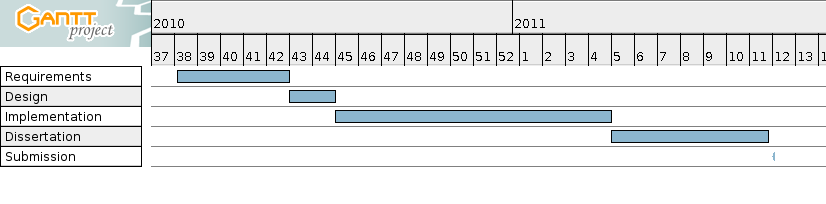
\includegraphics[width=14cm]{appendix/Diagrams/GIMplan.png}
        \caption{Gantt chart of our planned schedule.}
        \label{lockingDia}
    \end{center}
\end{figure}

\begin{figure}[!h]
    \begin{center}
        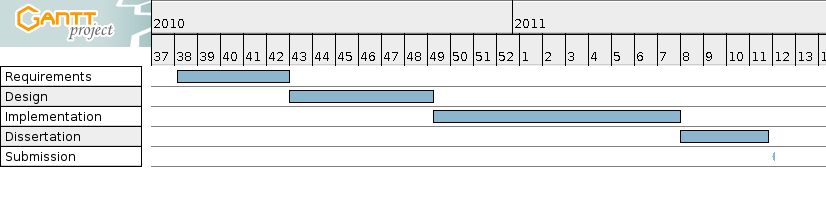
\includegraphics[width=14cm]{appendix/Diagrams/GIMreal.png}
        \caption{Gantt chart of our actual schedule.}
        \label{lockingDia}
    \end{center}
\end{figure}

The process of designing the system took longer than was initially anticipated, which delayed the implementation process significantly. The implementation process for basic functionality went smoothly and was finished relatively quickly, however a large amount of time was spent improving the interface and polishing the program. Our original plan provided almost 2 months to write this dissertation, in reality we had only 1 month.  

\section{Version Control}

For this project we used version control to manage code and documentation. All internal documentation was hosted using Google Docs, while this document and the java code was managed using SVN provided by Google Code. Our project initally used the SVN provided by the Computing Science school in Glasgow University, however, due to stability and relability issues we moved our project to Google's infrastructure.


\chapter{Status Report}
\documentclass{article}
\begin{document}

\section{Status}

\label{appenstatus}

The program is stable and does not appear to have any substantial bugs. The program meets the requirements outlined in the problem definition. \\

{\bf List of known issues with GIM:}
\begin{itemize}

\item{In some instances, a contact will come online and cause the users' contact list to stop displaying contacts. The user can fix this by selecting the "Display Offline Users" option.}

\item{A long line of text will necessitate the user to scroll across the chat area, as oposed to the text wrapping round.}

\item{The Block feature acts more like an ignore feature; the user that blocks a contact still appears online that contact.}

\item{If a user goes offline while talking to a contact, any messages that the contact sends while the user is offline will be send when they sign back online, assuming the contact remains online. This could be considered a feature of the system, as this it is a partial implementation of offline messages. As the user is not made aware that this will happen, the issue is considered a defect.}

\end{itemize}

\end{document}


\chapter{Summary Log}
\label{sumlog}

This document outlines the sections assigned to each team member. However, throughout the project we helped each other on our sections, so in some places the line between what person did what is more blurred.

{\bf James}:

Organisation: Version control, server hosting\\
Design: Server design, protocol specification architect\\
Implementation: Server, GUI friend list JList renderer, GUI user data listeners.\\
Report: Protocol design, server design, server implementation, protocol spec in appendix

{\bf Heather}:

Organisation: Quality assurance, report editor, planner, internal meetings manager.\\
Design: Interface design, requirements analysis, client structure\\
Implementation: GUI front-end, GUI back-end (some networking interface implementation)\\
Report: Introduction, problem definition, conclusion, GUI implementation section, chapter introductions, chapter summaries, editing. 

{\bf Ewan}:

Design: Interface design, requirements analysis\\
Documentation: Use cases, interface design (wire frames)\\
Implementation: GUI front-end\\
Report: Design of GUI, features, appendix

{\bf Gordon}:

Organisation: Team secretary\\
Design: Client structure, network component, some contributions to protocol specification\\
Implementation: Network component, GUI back-end (model and controller: creating windows, routing messages to windows, and managing chats between clients)\\
Report: Client design, networking design, client implementation, evaluation



%==============================================================================
\bibliographystyle{plain}
\bibliography{example}
\end{document}
